% !TEX root = ../spec_kernel_agent_main.tex
\section{Background}\label{sec:bg}

\begin{figure}[t]
    \centering
    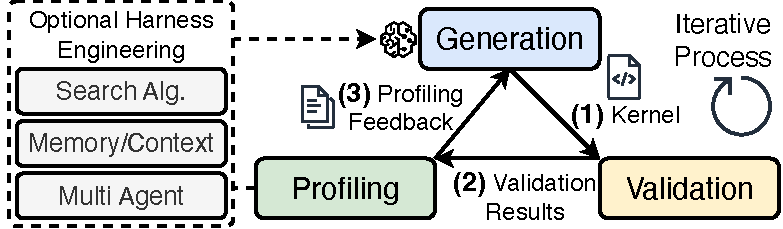
\includegraphics[width=\linewidth]{figs/agent_workflow.pdf}
    \vspace{-20pt}
    \caption{The three phases of agentic kernel optimization iteration: generation, validation, and profiling.}
    \label{fig:agentic_kernel_optimization}
    \vspace{-20pt}
\end{figure}

GPU kernel optimization is an iterative and verifiable task. Realizing a competitive kernel typically requires experts weeks per operator on a given GPU~\cite{Kernel-Smith,AlphaEvolve,cudal1,cudaagent}.

\noindent\textbf{Agentic Kernel Optimization} iteratively performs three phases as shown in Figure~\ref{fig:agentic_kernel_optimization} to generate and optimize kernels.
{\textbf{(1)} Generation} invokes the LLM on the accumulated context to produce a candidate kernel (e.g., CUDA/C++~\cite{kernelbench} or Triton~\cite{TritonBench}).
{\textbf{(2)} Validation} checks the candidate kernel for compilation, execution, and output correctness against a reference~\cite{kernelbench,TritonBench}. Any failure (compile error, runtime error, or numerical mismatch) is merged into the LLM's context to guide the next iteration's correction. Only kernels passing all three checks proceed to profiling.
{\textbf{(3)} Profiling} measures the candidate kernel's detailed performance metrics using NVIDIA Nsight Compute (\texttt{NCU}). The resulting metrics are merged into the LLM's context as feedback to guide subsequent generations.
Both validation and profiling require exclusive GPU access for measurement accuracy, since GPU sharing would distort both the speedup measured against the reference kernel and the profiled performance metrics.
Due to this exclusivity, existing frameworks statically dedicate one GPU per kernel to run its validation and profiling~\cite{cudaforge,TritonForge}, a partitioning we refer to as ``one GPU per kernel''.

\noindent\textbf{Harness Engineering Approaches} are also explored for agentic kernel optimization, including multi-agent collaboration~\cite{cudaforge,KernelSkill,Astra} and memory/context management~\cite{STARK,CuTeGen,K-Search}, evolutionary search~\cite{AlphaEvolve,openevolve,kernelagent2025,Kernel-Smith,KernelEvolve}, and verifier-guided search~\cite{ImprovingEfficiencyOfGPUKernelOptimizationAgents,AutoKernel,SwizzlePerf} to improve the kernel performance (Figure~\ref{fig:agentic_kernel_optimization} left). These works differ in their agentic optimization algorithms but still rely on the same three-phase iteration: invoking the LLM to generate kernels, validating their correctness against a reference, and profiling them for performance metrics.
Despite the rapidly evolving algorithmic frontier, the system-level efficiency of existing harness engineering approaches has received little attention. To analyze it, we characterize the agentic kernel optimization workload in \S\ref{sec:mot}.